\setcounter{chapter}{10}
\setcounter{section}{0}
\setcounter{figure}{0}
\setcounter{equation}{0}
\setcounter{table}{0}
\chapter*{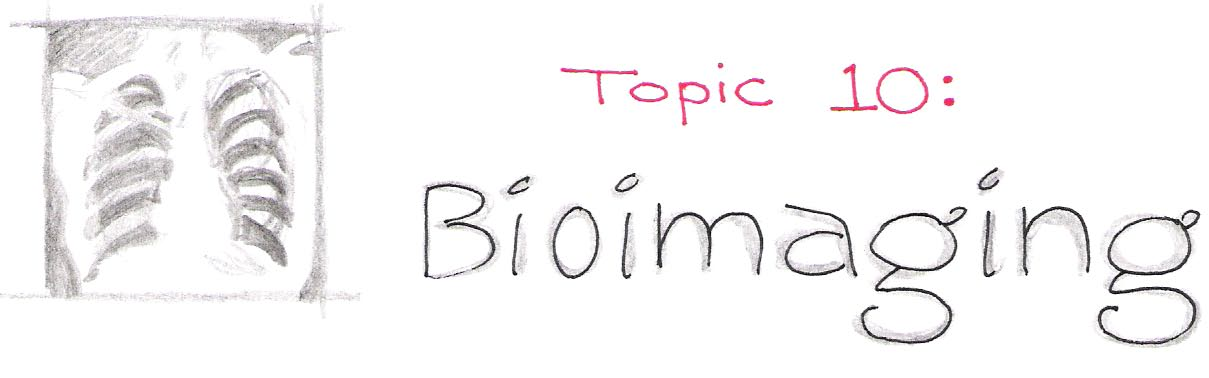
\includegraphics[width=\textwidth]{./figures/Topic10/Topic10.jpg}}
\addcontentsline{toc}{chapter}{Topic 10: Bioimaging}

\section{Introduction}

In the past few decades, basic biological research and diagnostic medicine have flourished as imaging techniques have improved.  We can now view proteins at work in the cell, scan the body for anomalies, and watch neurons firing in the brain.  Imaging techniques are numerous and diverse, but they can be roughly grouped into three categories according to the types of images they produce: anatomical, functional, and molecular.  Anatomical imaging techniques show shape and structure directly.  Functional imaging relies on recording tissue activity like oxygen consumption or glucose metabolism to create an image.  Molecular imaging provides visual insight into events that occur at the molecular level, like gene expression.  As we shall see, the distinction is often blurred, particularly between the latter two types.

This chapter will introduce the basic concepts behind some of the most widely-used types of bioimaging: microscopy, ultrasound imaging, and various types of tomography.


\section{Microscopy}

Microscopes are used to magnify small objects so that they may easily be seen by the eye.  A number of types of microscopes exist.  Light microscopes, invented in the Renaissance, are still the most commonly used form of imaging in the laboratory today.  Electron microscopes, developed in the 1950s, have made possible much greater resolution, i.e.the smallest detail that can be distinguished.  Newer types, like confocal scanning laser microscopes and scanning probe microscopes, allow imaging of complex specimens and even individual molecules.  The quality of any microscope depends on both its resolution and its overall magnification, which is how big the object appears relative to its actual size.  Light microscopes, which can typically achieve resolutions of 0.2 $\mu$m and magnifications around 1,000X. The resolution is limited by the diffraction of light through the objective much in the same way as the visual acuity in the eye is limited by the size of the pupil (Topic 5, Eq.~\ref{eqn5-7}):
$$D=\frac{1.22\lambda}{\theta},$$ 
where for a microscope $\theta$ is about 1.  Electron microscopes can magnify up to 100,000X and resolve at 5 $\text{\AA}$, over 100 times better than light microscopes. The higher resolution compared to light microscopes is directly attributed to the small size of the wavelength.  Finally, the scanning tunneling microscope magnifies a million times and can resolve individual atoms. Scanning tunneling microscopes use a microscopic probe that ``feels'' the surface through an electron current as it scans it and thus uses a radically different imaging principle.  Our discussion will focus primarily on light microscopy.

The basic principle behind all light microscopes is the same: one lens creates a magnified image of the sample, and a second lens magnifies the image of the first.  The first lens, called the objective, collects light from the sample (object) and projects it onto a plane inside the microscope.  If we were to place a piece of paper there, the image of the object would appear in focus and inverted upon it.  Optically, this image is called a real image.

The second lens is the eyepiece.  It functions like a magnifying glass, allowing the eye to focus on the nearby image.  For most microscopes, the first image of the sample is only a few centimeters away from the eye, so the eyepiece both makes viewing more comfortable and provides added magnification.  Figure 1 illustrates the two components of a microscope.  
\begin{figure}[!htb]
	\centering
	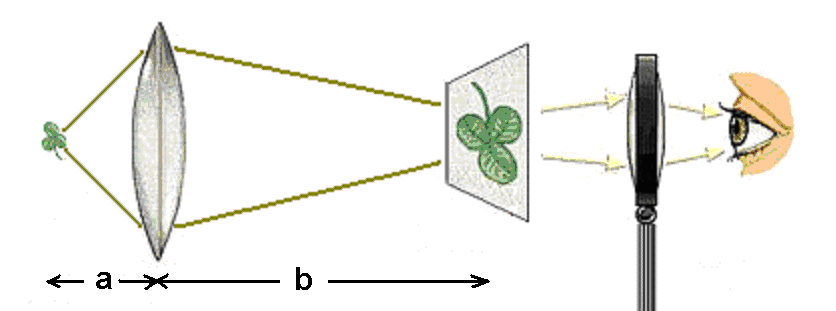
\includegraphics[width=3.5in]{./figures/Topic10/Fig10-1.png}
	\caption{A light microscope consists of two lenses, the objective and the eyepiece.}
	\label{Fig10-1}
\end{figure}

Recall from Topic 5 that $a$ and $b$, the object distance and image distance respectively, are related to the focal length $f$ of the lens by the equation $1/f=1/a+1/b$. The distance $a$ from the object to the objective lens is typically short, usually less than a centimeter, whereas the distance $b$ from the lens to the image plane is on the order of tens of centimeters.  The magnification of the image is given by the ratio $b/a$.  Therefore, using typical distances for these quantities, we can expect the magnification associated with the objective lens to be 10 to 100X.

The second step of magnification uses the image located a few centimeters away from the eyepiece to generate a second (virtual) image located tens of centimeters away.  The additional magnification from this step is equal to the ratio of these two distances, so the eyepiece magnifies the image by 10X or more. The overall magnification of the microscope, then, is the product of the individual magnifications of the objective and the eyepiece.  Light microscopes can easily achieve overall magnifications of 100X and, depending on the quality of the lenses, as high as 1,000X.

Many types of light microscopes exist, including bright-field, fluorescence, phase-contrast, and confocal.  We will focus on the brightfield and fluorescence techniques, as they are the most widely used in biological research.

Bright-field microscopy is the most common of all types.  Light from a lamp in the microscope shines up through the sample, forming an image where regions of the sample absorb or scatter light.  This is similar to how light passing through a transparency placed on an overhead projector creates an image on a screen.  One drawback to bright-field microscopy is the poor contrast between cellular features because most cellular structures absorb very little light. To enhance these features, researchers often stain samples with strongly-absorbing dyes.    
Further enhancement of cellular components can be achieved with fluorescence microscopy.  Here, the sample is incubated with fluorescent dyes called fluorophores (or fluorochromes), before being placed under the microscope.  The fluorescence emitted by fluorophores generally occurs at wavelengths close to those at which they absorb and is relatively weak. Therefore careful wavelength filtering is required to insure that excitation light does not interfere with the observation of fluorescence. As depicted in Fig.~\ref{Fig10-2}, light from a bright lamp (typically a lamp containing mercury or xenon at high pressure) is filtered by filter A to a narrow range of wavelengths that are optimized to excite a particular fluorophore. These wavelengths are reflected onto the sample by a special mirror (C) called a dichroic (from the greek ``two colors'', more about this below). The reflected light shines on the sample, which scatters much of it back; some of it is absorbed by the fluorophore, which responds by fluorescing at a slightly higher range of wavelengths than they absorb.  Both wavelength ranges are collected by the objective and directed toward the detector. Along the way it encounters the same dichroic mirror, which reflects the scattered light preferentially while allowing the fluorescence at longer wavelengths to pass through. Since the color separation at the dichroic is not perfect, a small portion of the excitation light can leak through it. Although small in proportion to what illuminated the sample, the scattered light is can still be much more intense than the fluorescence. To avoid overwhelming the detector with this undesired light signal, a second filter (B) is used. Thus, with a proper combination of filters and dichroic, the resulting image shows a pattern of fluorescence that appears to be glowing on a black background.  
\begin{figure}[!htb]
	\centering
	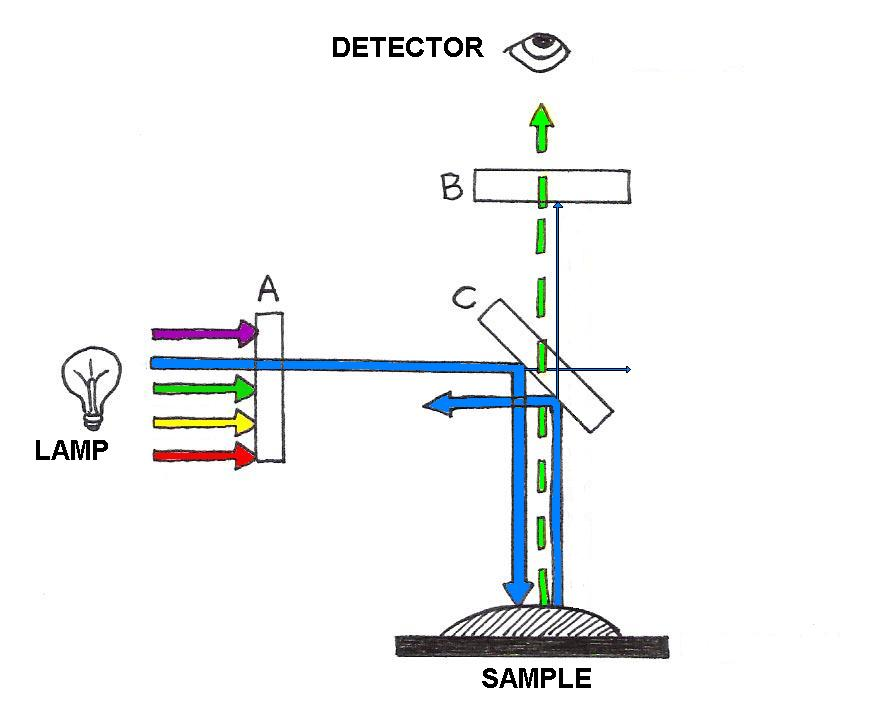
\includegraphics[width=4.0in]{./figures/Topic10/Fig10-2.jpg}
	\caption{ Fluorescence microscopy is achieved with the aid of wavelength-selective filters.  These filters select a narrow range of wavelengths for illumination of a sample, and separate the fluorescence from the portion of the illumination scattered by the sample.}
	\label{Fig10-2}
\end{figure} 

\section{Ultrasound Imaging}

Ultrasound imaging, used to image internal organs and perform noninvasive prenatal exams, works by using higher frequencies of sound than can be heard by the human ear.  It is essentially the same as sonography, which is used for navigation both by bats hunting for food and by submarines and dolphins maneuvering around underwater obstacles.  Based on the pulse-echo principle, an ultrasound probe emits very short pulses of high-frequency sound waves and detects the reflected waves (echoes) that bounce off of internal surfaces, like the surfaces of bones or organs.

The arrival time of the echo provides information about the distance from the probe to the obstacle, while the orientation of the detector provides information about the direction of the obstacle.
\begin{figure}[!htb]
	\centering
	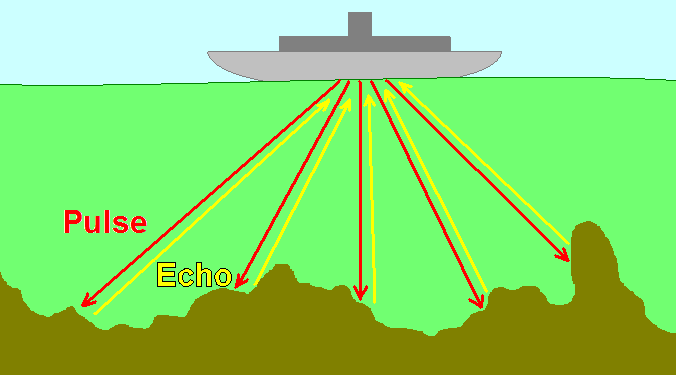
\includegraphics[width=4.0in]{./figures/Topic10/Fig10-3.png}
	\caption{The pulse-echo principle used in medical imaging is that same as that used in underwater navigation.}
	\label{Fig10-3}
\end{figure} 
The same technique can be used to probe biological tissues: by determining the time delay from pulse emission to echo detection, one can determine the depth of reflecting tissue layers. Furthermore, by knowing the acoustical impedance (discussed in Topic 3) of each layer, we can even determine the percent of the ultrasound intensity that is reflected by each of those layers. The reflectivity aids us in characterizing which type of tissue is reflecting the ultrasound waves. A typical ultrasound scan is shown below in Fig.~\ref{Fig10-4}. 
\begin{figure}[!htb]
	\centering
	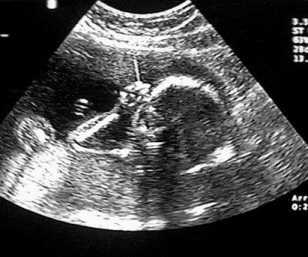
\includegraphics[height=2.0in]{./figures/Topic10/Fig10-4a.jpg}
	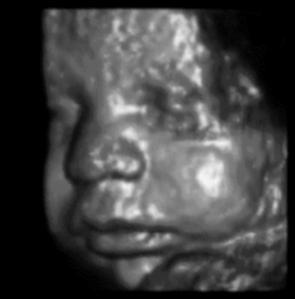
\includegraphics[height=2.0in]{./figures/Topic10/Fig10-4b.jpg}
	\caption{A typical 2D real-time image obtained during an ultrasound scan (left) and a 3D reconstruction derived from multiple 2D scans (right).}
	\label{Fig10-4}
\end{figure} 

As an example, suppose you want to determine the depth of a bone beneath the skin and its reflectivity to ultrasounds. Let us say that the pulse-echo time delay is 4.0 $\mu$s and assume for simplicity that skin and muscle layers exhibit the same properties as water (same propagation speed and same acoustical impedance.)  Let us perform the calculations using the properties that are summarized in Table \ref{table10-1}.
\begin{table}![h]
\begin{center}
\begin{tabular}{|l|c|c|c|}
\hline
Material & Density ($\times10^{-3}$kg/cm$^3$) & Velocity (m/s) & Impedance $\times10^{-6}$ (kg/m$^{-3}\cdot$ s) \\
\hline
Water & 1000 & 1,480 & 1.48\\
Muscle & 1080 & 1580 & 1.71\\
Fat & 900 & 1450 & 1.30\\
Brain & 1050 & 1540 & 1.62\\
Blood & 1030 & 1570 & 1.62\\
Bone & 1850 & 3500--4300 & ~7\\
\hline
\end{tabular}
\caption{Properties of sound waves in various media.}
\label{table10-1}
\end{center}
\end{table}
If $d$ is the depth of the bone, the pulse and echo must travel a total of $2d$ in $4.0\times10^{-6}$ s.  Since distance = velocity $\times$ time, we can solve for $d$: 
\begin{align}
2d &= (1500~{\rm m/s})(4.0\times10^{-6}~{\rm s}) = 0.0060~{\rm m}\nonumber\\
d &= 0.0030~{\rm m~or}~3.0~{\rm mm}.\nonumber
\end{align}
Thus, the bone is located 3 mm below the skin.

Now let us calculate the percentage of pulse intensity picked up by the detector.  The sum of signal reflection and transmission must equal 100\%, so to find the percent reflected we simply find $R = 1 -T$.  Recall from Topic 3 that percent transmission
$$T = \frac{4\frac{\mathcal{Z}_w}{\mathcal{Z}_{bone}}}{\left(1+\frac{\mathcal{Z}_w}{\mathcal{Z}_{bone}}\right)^2}.$$
Using the data in Table \ref{table10-1}, we find that
\begin{align}
R &= 1-\frac{4\cdot\frac{1.48}{7}}{\left(1+\frac{1.48}{7}\right)^2}\nonumber\\
R &= 0.42\nonumber
\end{align}
The example shows that bones reflect a significant portion of the incoming ultrasound intensity, which explains why they are seen so well under this form of imaging.  However, the contrast between other tissues is usually much smaller. For example, the reflection at the interface between fat and muscle tissues ($\mathcal{Z}_{\rm fat}/\mathcal{Z}_{\rm muscle} = 1.3/1.71$) gives only 2\% reflection. 

What determines the resolution of an ultrasound image?  There are actually two types of resolution associated with this technique: depth (or axial) resolution and lateral resolution. The depth resolution, as the name implies, is related to how well the technique can resolve depth. One way to quantify this is to test the ability of the technique to separate two objects that have different depths, as illustrated in Fig.~\ref{Fig10-5}. 
\begin{figure}[!htb]
	\centering
	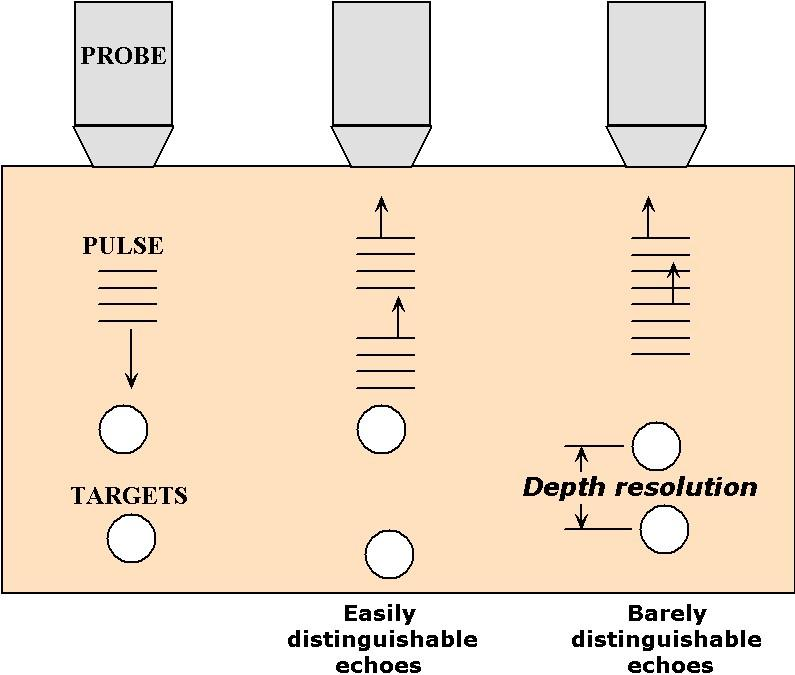
\includegraphics[height=3.0in]{./figures/Topic10/Fig10-5.jpg}
	\caption{An illustration of the relationship between pulse duration and depth resolution in ultrasound imaging.}
	\label{Fig10-5}
\end{figure}
As the depth difference becomes smaller, the echoes that reflect from them come closer to each other in time; when they begin to overlap in time the detector can no longer distinguish the two as separate echoes. This is the limit of depth resolution. Hence, depth resolution depends on two inter-related factors: the closeness of the objects and the duration of the pulses generated by the ultrasound source.  For this reason, it is important to use pulses as short-lasting as physically possible. Using waves of frequency $f$, the shortest pulse duration that can be produced is typically equal to one period of oscillation, or $1/f$.   Thus, ultimately, the depth resolution depends on the frequency used.

To estimate this resolution, simply calculate the depth reached during a round-trip time corresponding to the pulse duration, that is $2d={\rm  c} (1/f)$. This yields a depth $d$ of c/2$f$. Sonographs used by submarines or ships operate at frequencies around 10,000 Hz.  Since the speed of sound in water is approximately 1,000 m/s, these sonographs resolve as small as 0.1 m.  This kind of resolution is adequate for navigation around underwater obstacles. In medical sonography, often used to examine fetal development, it is necessary to resolve much smaller details.  Here the resolution must fall below 1 mm, demanding frequencies greater than 1 MHz!
  
Lateral resolution refers to the ability to resolve two objects located side-by-side at the same depth. This type of resolution depends on the width of the ultrasound beam, because when the objects are separated by a distance smaller than the width of the beam that scans them, they cannot be distinguished. This concept is illustrated in Fig.~\ref{Fig10-6}
\begin{figure}[!htb]
	\centering
	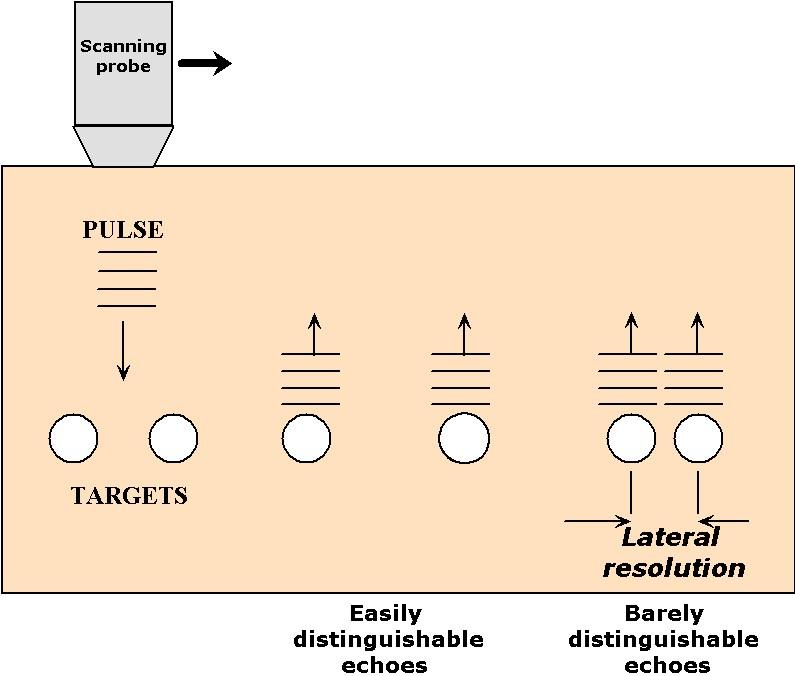
\includegraphics[height=3.0in]{./figures/Topic10/Fig10-6.jpg}
	\caption{An illustration of the relationship between pulse width and lateral resolution in ultrasound imaging.}
	\label{Fig10-6}
\end{figure}
Narrow ultrasound beams can be produced by small ultrasound transducers but, due to diffraction (see Topic 5), their widths tend to spread out rapidly as soon as they propagate away from the transducer. The divergence of the beam width follows equation \ref{eqn5-7} of Topic 5, $\theta = 1.22\lambda/D$, where here $D$ is the diameter of the ultrasound transducer and $\lambda$ is the wavelength of the wave in the medium (also equal to c/$f$). Therefore, for a frequency of 1 MHz, a propagation velocity of 1500 m/s, and a diameter of 1 mm, the divergence angle is about 1.8 radians. This implies that the radius of the beam increases by a 1.8 mm for every mm of penetration. Such a spread of waves makes it nearly impossible to resolve lateral detail, particularly for depths beyond a few mm. For neonatal applications, where the scanner must image to depths of 10 cm or so, a better approach is to adopt a wider transducer (~1 cm) in combination with a higher frequency ($\sim$5 MHz). This combination results in a much smaller divergence angle ($\sim$ 0.036 rad), that is in a beam for which the radius increases by only 0.036 cm for every cm of propagation.   
 
\section{Tomography}

The earliest form of medical imaging was probably the x-ray picture, which is still widely used today.  When x-rays transmitted through the body are captured on x-ray-sensitive film, they reveal ``shadows'' cast by different tissues.  A major drawback to this technique is the confounding patterns obtained when two or more tissues cast their shadow in the same place, particularly when one of them is a strongly-absorbing tissue such as bone. In such instances a clearer diagnosis could be obtained if one could isolate the image produced from a single depth (i.~e.\,, a cross-section) from all the others in the body.

In the latter part of the twentieth century, innovations in technology and image analysis brought to fruition medical scanners that literally provide cross-sections of the body non-invasively, that is, without ever cutting the body open. The first of these methods, also known as x-ray Computed Tomography(CT), takes projections collected from different perspectives around the body and combines them mathematically to generate cross-sections of the body. Later, other methods emerged that obtained cross-sections of the body using other forms of energy. The principle behind these different forms of imaging, or imaging modalities, are discussed next.

\subsection{X-Ray Computed Axial Tomography (CAT)}

CAT scanners (also called Computed Tomography, or CT, scanners) were the first tomographic scanners developed for medical applications.  They use an array of x-rays beams projected from many angles around the body to create anatomical images like the one below.
\begin{figure}[!htb]
	\centering
	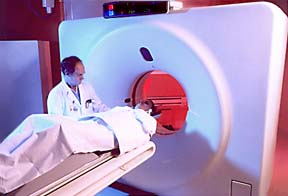
\includegraphics[height=2.0in]{./figures/Topic10/Fig10-7a.jpg}
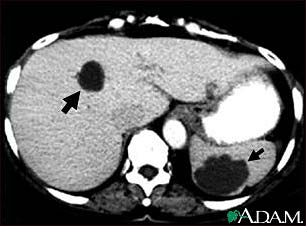
\includegraphics[height=2.0in]{./figures/Topic10/Fig10-7b.jpg}
	\caption{Cysts in the liver and spleen appear in a CAT scan image.  Image from \href{http://health.allrefer.com/health/polycystic-kidney-disease-liver-and-spleen-cysts-ct-scan.html}{http://health.allrefer.com/health/polycystic-kidney-disease-liver-and-spleen-cysts-ct-scan.html}.}
	\label{Fig10-7}
\end{figure}

To understand the basic idea behind CAT scans, consider the illustration in Figure \ref{Fig10-7}, in which an unknown object is positioned in front of two illuminated screens.  
\begin{figure}[!htb]
	\centering
	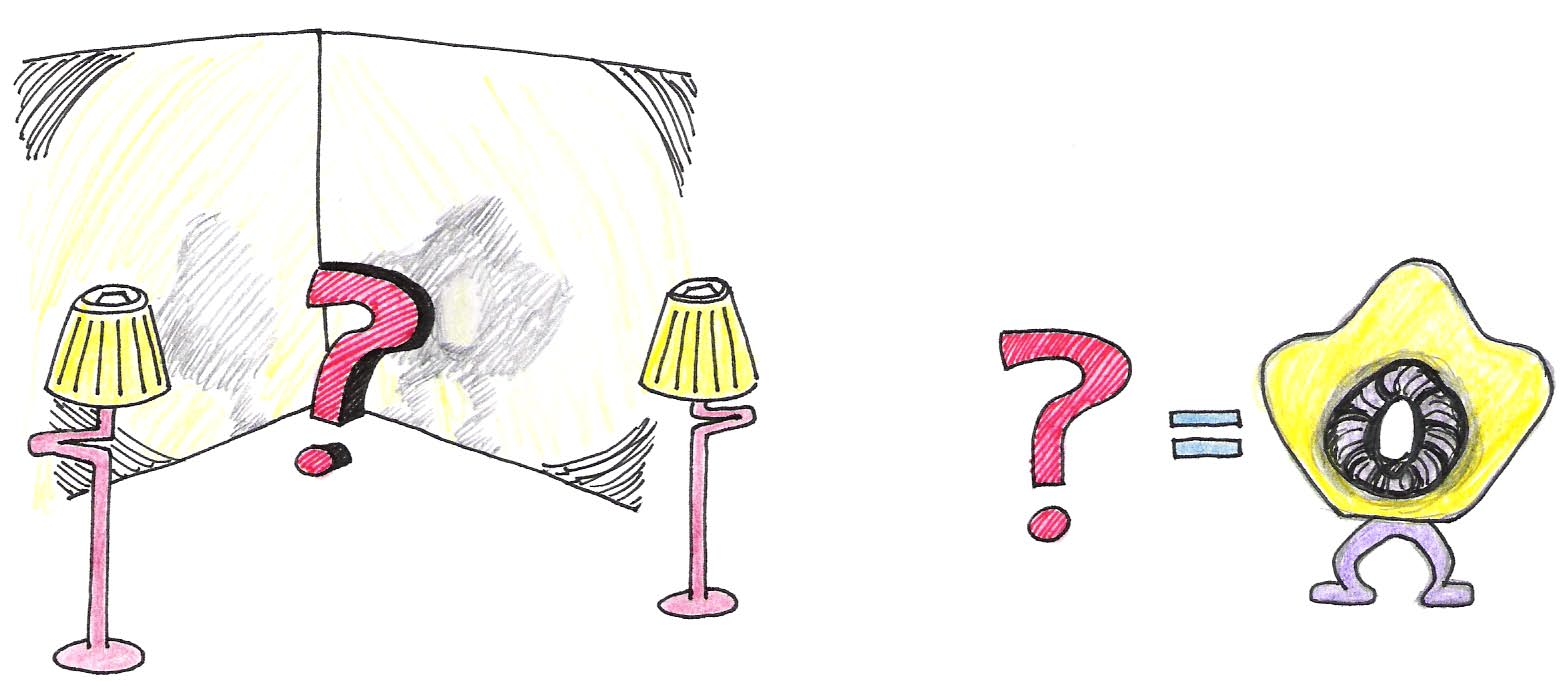
\includegraphics[width=\textwidth]{./figures/Topic10/Fig10-8.jpg}
	\caption{Together, the two shadows give a better representation of the object.}
	\label{Fig10-8}
\end{figure}
If the light source is directly in front of the object, we can see in its shadow a hole through its center, but know nothing of its thickness.  If the light source is on his left, we see by its shadow that it has a rounded protrusion in the area where the hole in the other shadow is located.  Neither shadow provides enough information by itself, but when they are viewed together, our brains can reconstruct the most probable shape of the object.  In the same way, as illustrated in Figs.~\ref{Fig10-8} and \ref{Fig10-9}, a CAT scanner compiles the x-ray shadows from many line scans known as projections, and reconstructs from those the interior of the slice.  
\begin{figure}[!htb]
	\centering
	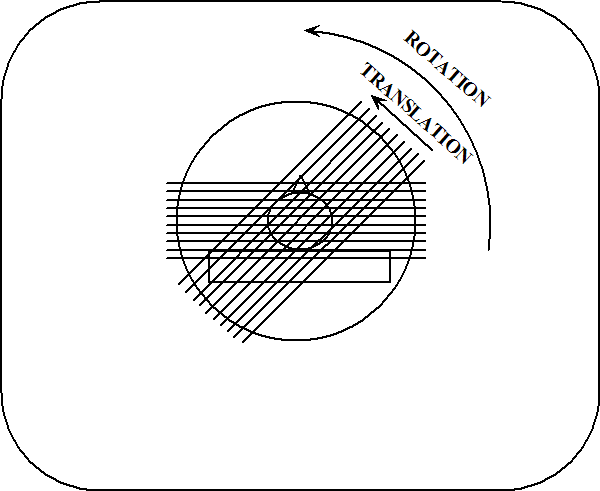
\includegraphics[width=3.0in]{./figures/Topic10/Fig10-9.png}
	\caption{Two x-ray projections taken during a CAT scan.}
	\label{Fig10-9}
\end{figure}
Each projection is completed at a different angle, and the resulting shadows are recorded by a computer.  As shown in Fig.~\ref{Fig10-9}, a projection is represented mathematically as a profile of x-ray absorption values along points $s_i$ in each of the directions $\theta_i$.

\begin{figure}[!htb]
	\centering
	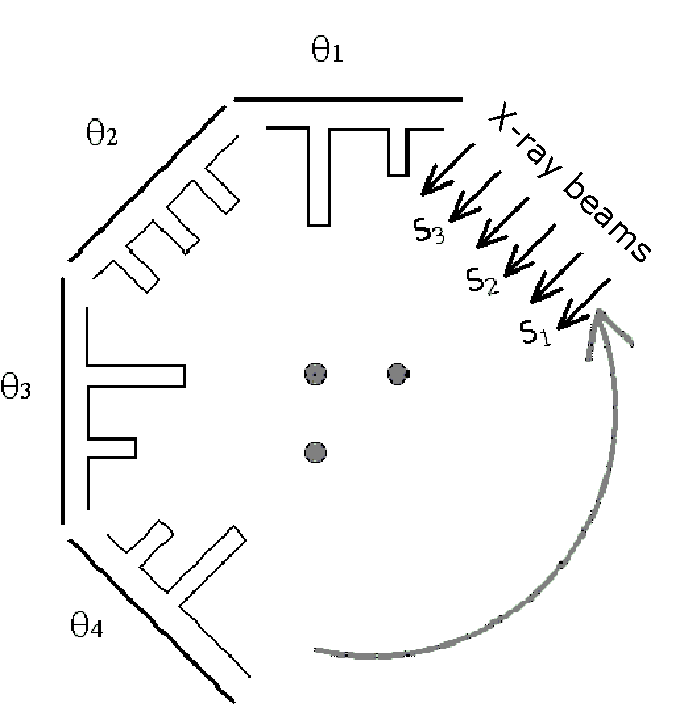
\includegraphics[width=3.0in]{./figures/Topic10/Fig10-10.png}
	\caption{The bar-graphs represent x-ray absorption at the detector opposite the x-ray source.}
	\label{Fig10-10}
\end{figure}
The dots in Fig.~\ref{Fig10-10} represent the horizontal cross-section of a three cylindrical object, such as bones sticking up out of the page. The bar-graphs in Figure \ref{Fig10-10} represent the level of attenuation (or absorption) that x-rays experience when they pass through the dots. For example, when a ray passes through two dots they experience twice the absorption value compared to those that only pass through one of the dots.  No absorption occurs where the x-rays do not pass through any of the dots.
  
After the absorption profile information is collected, it must be analyzed to reconstruct the image of the sample, just as our brain used the two shadows of the object in Figure \ref{Fig10-8}.  Several mathematical techniques can be used to reconstruct the interior of the object. Here we discuss a conceptually easy one known as a back-projection, which is illustrated in Fig.~\ref{Fig10-11}.  According to this technique, the absorption values from each scan are ``projected'' back into the sample: this means that each point along a projection path (defined by both $s$ and $\theta$) gets assigned the same average value.  When this step is complete, the back-projected values are summed up at each point within the plane of the slice.  It follows from this approach that points with higher values are indicative of regions of higher attenuation. Figure \ref{Fig10-11} illustrates the idea of back-projection for the sample in Figure \ref{Fig10-10}.  
\begin{figure}[!htb]
	\centering
	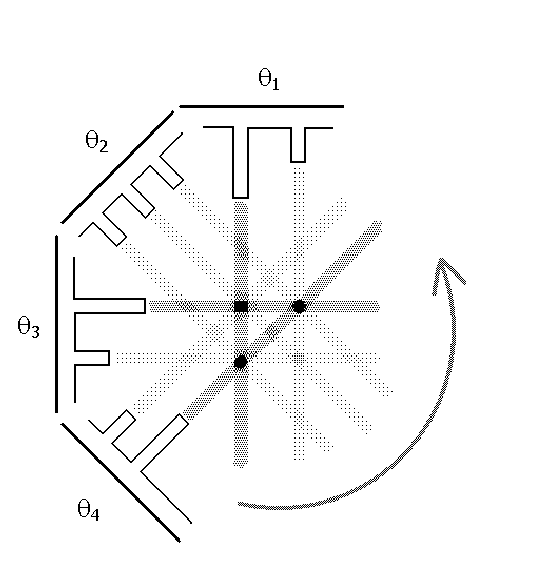
\includegraphics[width=3.0in]{./figures/Topic10/Fig10-11.png}
	\caption{An illustration of the back-projection technique.}
	\label{Fig10-11}
\end{figure}
Notice that this method is not perfect--the attenuation gets ``smeared'' over the sample, or spread out.  Furthermore, ``ghosts'' can also appear where the back-projection creates a false conversion of beams, such as the one shown in Fig.~\ref{Fig10-11}- opposite to the location of the dots. One feature about these faint ghosts is that they will appear in more locations when the sample is probed from a larger number of angles. Eventually, when the number of angles is large enough, the distribution of ghosts will appear smooth enough to appear as a uniform background that does not stand out.

To get a better feel for the mathematics involved, let us work a very simple example.  Consider a two-dimensional sample, a square, divided equally into nine smaller squares.  Each square is labeled with a number that indicates its relative density.
\begin{table}[!h]
\begin{center}
\begin{tabular}{|c|c|c|}
\hline
0 & 0 & 3\\
\hline
0 & 0 & 0\\
\hline
3 & 0 & 0\\
\hline
\end{tabular}
%\caption{}
\label{table10-2}
\end{center}
\end{table}
We might think of 3 as representing bone and 0 as representing surrounding tissue. To get all the necessary information, we need to do scans from four different angles.  We sum up the values for each line scan from each angle, yielding a total of twelve values:  
\begin{figure}[!htb]
	\centering
	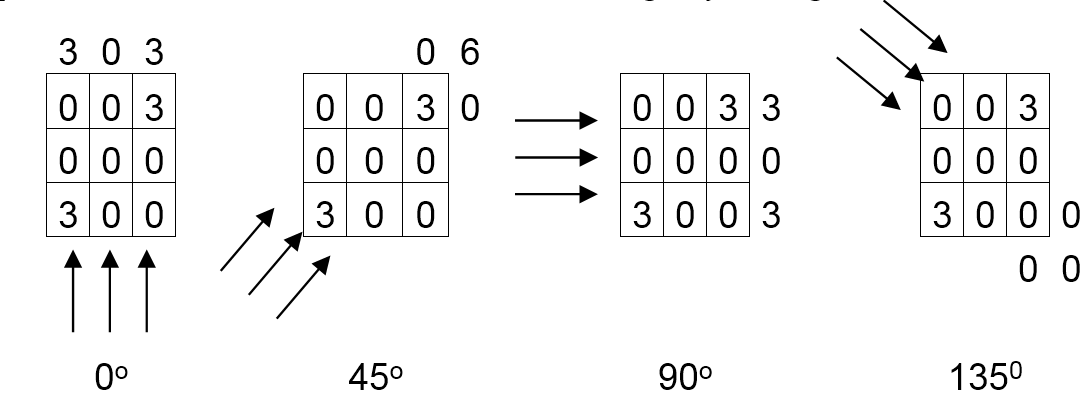
\includegraphics[width=\textwidth]{./figures/Topic10/CTExample1.png}
	%\caption{}
	\label{CTEx1}
\end{figure}
Now we are ready to do a simple back-projection.  First we divide the sums attained above by the number of boxes that have contributed to each scan, which in each case here is either two or three.  Then we place the resulting value in each square along the projection line. Finally, we add up the four values for each of the nine squares to arrive at the final image.  
\begin{figure}[!htb]
	\centering
	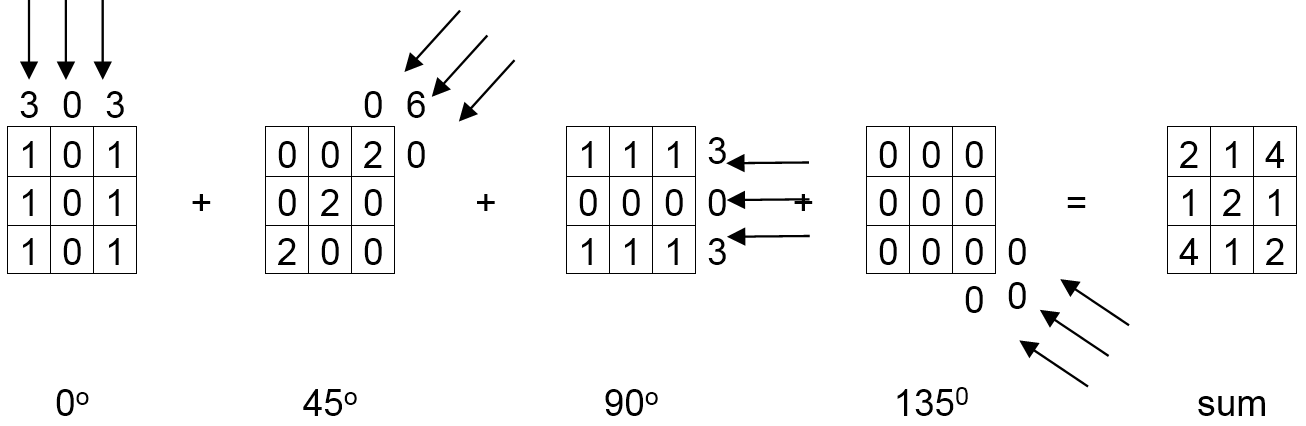
\includegraphics[width=\textwidth]{./figures/Topic10/CTExample2.png}
	%\caption{}
	\label{CTEx2}
\end{figure}
Compare the final image to the original sample.  Some areas appear to be absorbing x-rays where they should not be, but the highest values are indeed found where they should be, in the upper right and lower left boxes.

Is there an easy way to remove the unwanted absorption from the image so that it better represents the object?  Yes, but this so-called filtered back-projection requires more calculation.  It works by subtracting off extra-high values from adjacent boxes by using a multiplier.  To see what this means, we will work through the filtered back-projection for the example above, using multipliers of 1 for the centerline and -0.45 for the side lines.

We start with the first scan taken at 0$^{\circ}$ (upwards through the left-hand column).  The sum is 3, and since there are three boxes over which to distribute this value, each square gets an initial value of 1.  Before we assign the values, though, we apply the multipliers: the values in the left-hand column (the current centerline) are multiplied by 1, so that they remain the same.  The values on either side of the column (here, only the values in the middle column since there is no column to the left) take on the value of -0.45 times the value of the centerline boxes.  The result is shown below.\begin{figure}[!htb]
	\centering
	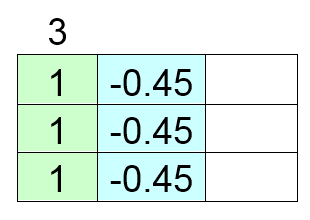
\includegraphics[width=2.0in]{./figures/Topic10/CTFilter1.png}
	%\caption{}
	\label{CTFil1}
\end{figure} 

We carry out the same procedure for the middle and right-hand columns in the same way.
\begin{figure}[!htb]
	\centering
	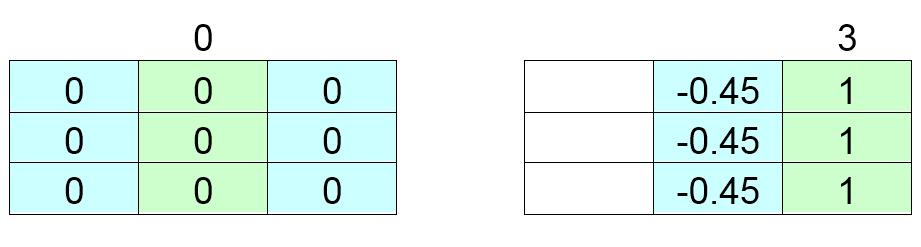
\includegraphics[width=\textwidth]{./figures/Topic10/CTFilter2.png}
	%\caption{}
	\label{CTFil2}
\end{figure}
Next we go on to the second scan, taken at 45$^{\circ}$.  The same calculations are performed.  
\begin{figure}[!htb]
	\centering
	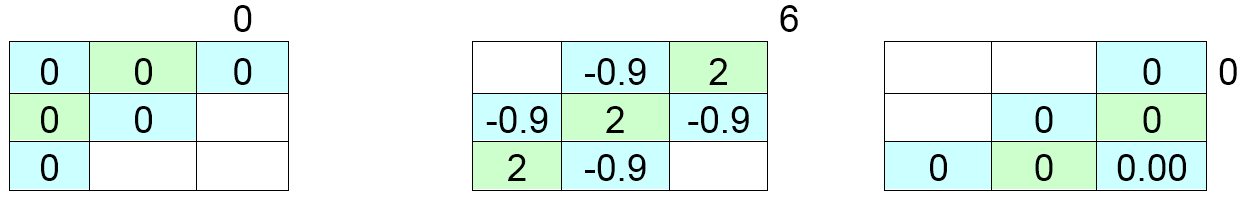
\includegraphics[width=\textwidth]{./figures/Topic10/CTFilter3.png}
	%\caption{}
	\label{CTFil3}
\end{figure}
After we do this for the third and fourth scans (90$^{\circ}$ and 135$^{\circ}$; not shown), we have twelve values for each of the nine boxes in the sample.  We add these twelve values to reach our final filtered back-projection:
\begin{table}[!h]
\begin{center}
\begin{tabular}{|c|c|c|}
\hline
2 & -0.8 & 4\\
\hline
-0.8 & 0.2 & -0.8\\
\hline
4 & -0.8 & 2\\
\hline
\end{tabular}
%\caption{}
\label{table10-3}
\end{center}
\end{table}

The result is much better than the simple back-projection; the areas where the sample absorbed x-rays the most are still clearly identified, but the surrounding areas drop to negligible values.  The technique is not perfect, as we still see ghosts in the upper left and lower right corners, but those would likely be reduced if we had probed the sample at additional angles.

\subsection{Positron Emission Tomography (PET)}

PET was the first form of tomography that made possible functional imaging.  Like CAT scanners, PET scanners make use of high-energy radiation to collect imaging data.  Instead of shooting x-rays through the body, however, PET scanners detect gamma rays (higher energy photons than x-rays) that are emitted from the body. Before a scan, the patient is given a substance such as oxygen gas or a glucose solution containing a radioactive isotope, like $^{15}$O or $^{18}$F. During their nuclear decay, these isotopes emit a particle called a positron. Positrons are the anti-matter version of protons, i.e. they ahev the same mass as an electron but they are positively charged. When substances containing these isotopes are metabolized by the body they are deposited at the site of metabolism from where they emit positrons. These particles are annhihilated as soon as they encounter their anti-matter counterpart, the electron, and in their place two gamma rays emerge. Their mass is converted to energy, resulting in two gamma rays that propagate in opposite directions (due to conservation of momentum). When this happens, two gamma rays can be detected simultaneously on opposing sides of the body, as shown in Fig.~\ref{Fig10-12}.  Because of the high density of electrons in the body, a positron can only travel several millimeters through tissue before being annihilated. 
\begin{figure}[!htb]
	\centering
	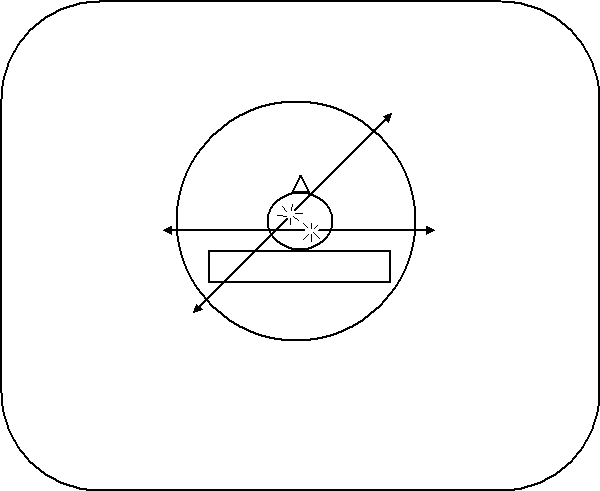
\includegraphics[width=3.0in]{./figures/Topic10/Fig10-12.png}
	\caption{Radioactive isotopes release positrons during decay, which annihilate electrons, forming two gamma rays traveling in opposite directions.  Here, two annihilation events occur in different areas of the brain.}
	\label{Fig10-12}
\end{figure}

The scanning device detects photons arriving on opposite sides of the sampling chamber at the same time.  When this happens, we know that the isotope must have been present in the line connecting the two points of detection.  After collecting information about the many lines resulting from positron emission, computers use the data to reconstruct the interior of the body.  These lines provide the same kind of information that x-ray beams in CAT scanners do--the mathematical techniques are almost the same.  Whereas CAT scanners measure absorption of x-rays external to the body, PET scanners compile images of gamma ray emission from within the body. These images reflect sites where the radioisotopes were metabolized in the body. A common indicator used in PET imaging is $^{18}$F-labelled fluorodeoxyglucose, a fluorinated version of glucose that is metabolized by cells as is glucose. Therefore cells with elevated levels of metabolism  such as activated brain tissue or tumors accumulate $^{18}$F to greater extents than others and therefore ``glow'' more intensely under this form of imaging. For this reason PET imaging is often categorized as a form of functional imaging since its images reflect tissue activity, whereas CAT scanners provide only structural information.

PET imaging has been widely used by neuroscientists to better understand what areas of the brain are activated for a variety of mental tasks and for diagnosis of brain diseases. An example of the latter is shown below in Fig.~\ref{Fig10-13}. Two brain scans demonstrate drastically different levels of metabolic activity between a normal brain and that of an Alzheimer’s patient.
\begin{figure}[!htb]
	\centering
	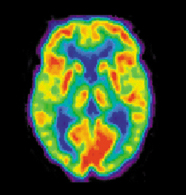
\includegraphics[width=2.5in]{./figures/Topic10/Fig10-13a.png}
	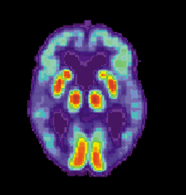
\includegraphics[width=2.5in]{./figures/Topic10/Fig10-13b.png}
	\caption{PET scans of a normal brain (left) and an Alzheimer’s Disease brain (right).  Image from \href{http://www.alzheimers.org/unraveling/07.htm}{http://www.alzheimers.org/unraveling/07.htm}.}
	\label{Fig10-13}
\end{figure}	 
 
\subsection{Magnetic Resonance Imaging (MRI)}

MRI is perhaps the most useful type of tomography, providing excellent anatomical images without exposing patients to potentially harmful radiation.  Figure \ref{Fig10-13} shows an MRI cross-section of the head.
\begin{figure}[!htb]
	\centering
	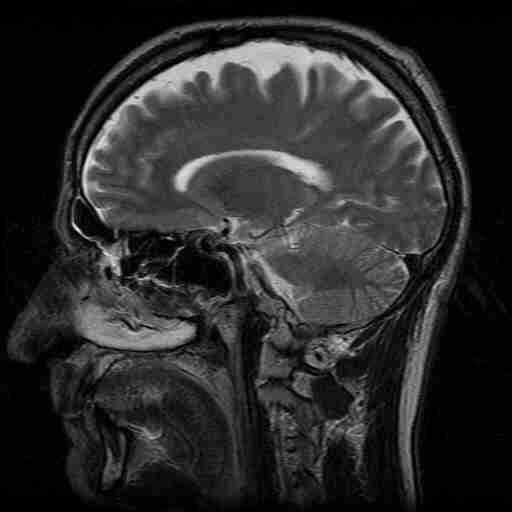
\includegraphics[width=3.0in]{./figures/Topic10/Fig10-14.jpg}
	\caption{MRI of the head.}
	\label{Fig10-14}
\end{figure}
MRI is fundamentally the same as Nuclear Magnetic Resonance (NMR), a research tool used to determine the structure of proteins and other large molecules.  (The technique simply has a different name when used in medical imaging because the term ``nuclear'' tends to frighten people.)  Since the theory of NMR is covered in depth in Topic 9, we will only hit the highlights as they relate to MRI in particular.  The magnetic field strength used in MRI scanners is typically on the order of 1--2 Teslas, resulting in a nuclear magnetic resonance frequency near 100 MHz.  This frequency is much lower than research-grade NMR machines, which operate between 500-900 MHz.  The lower frequency is adequate for MRI because these scanners need only detect the water content of tissues, unlike NMR scanners which must be able to differentiate among protons located within a molecule.

Under the influence of a uniform magnetic field, every proton in a water molecule resonates with the same frequency and therefore produces a signal that cannot be distinguished from the others around it.  
\begin{figure}[!htb]
	\centering
	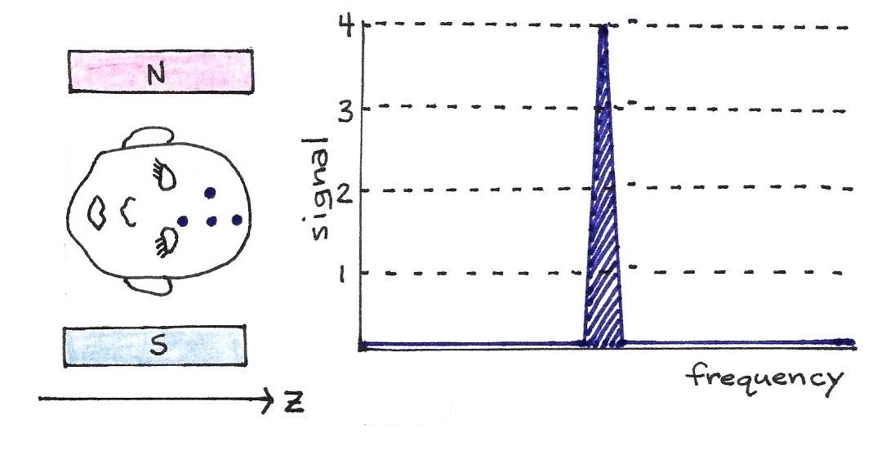
\includegraphics[width=4.0in]{./figures/Topic10/Fig10-15.png}
	\caption{The four dots on the man’s head represent four hydrogen atoms.  If the magnetic field is constant, as pictured, all four protons resonate at the same frequency, though they have different locations along the $z$-axis.}
	\label{Fig10-15}
\end{figure}
Since this does not allow differentiation between magnetic dipoles at different locations, it is not useful for imaging purposes.  Instead, MRI scanners use a magnetic field that gradually increases in strength along its $z$-axis.  Protons in a plane perpendicular to the stronger end of the magnetic field resonate at a higher frequency than those in a plane perpendicular to the weaker end.  Thus, it is possible to select a subset of magnetic dipoles--a slice of the body--to image by tuning the pulse frequency.
\begin{figure}[!htb]
	\centering
	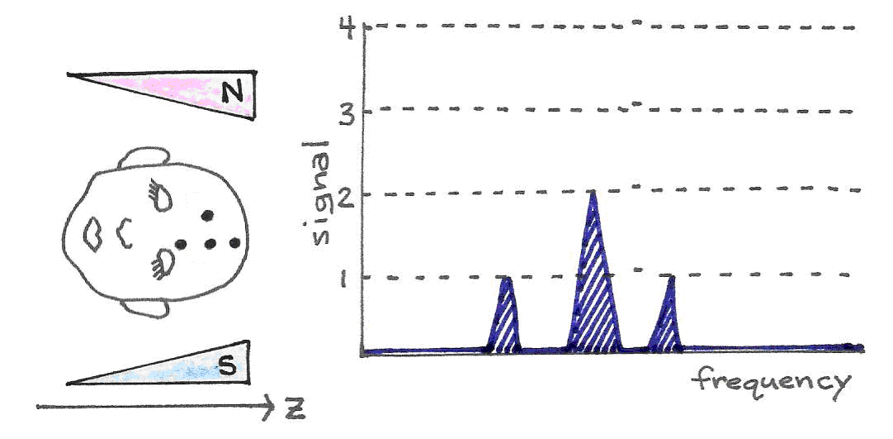
\includegraphics[width=4.0in]{./figures/Topic10/Fig10-16.png}
	\caption{With a gradually increasing magnetic field, the protons in the stronger region of the field resonate at a higher frequency than do the single protons in the weaker part of the magnetic field.  The signal strength is proportional to the number of resonating protons.}
	\label{Fig10-16}
\end{figure}

There are several steps in the scanning procedure.  After the patient is introduced into the scanner with a magnetic field gradient along the $z$-axis, a slice of the body perpendicular to the $z$-axis is chosen to image.  A radio-frequency (RF) pulse of the appropriate frequency is applied, which sets in motion all the dipoles within the slice.  Then each dipole is tagged according to its spatial coordinate ($x$, $y$) by two further steps: phase encoding along the $y$-axis and frequency encoding along the $x$-axis.

In phase encoding, a magnetic field gradient is applied momentarily in the $y$-direction.  This causes the already oscillating spins to increase their frequency to different extents depending on their location relative to the $y$-axis gradient field.  Again, the frequency of those dipoles closer to the stronger portion of the magnetic field increases more than the frequency of those near the weaker portion.  As the gradient field is turned off, the spins return to the same rotation frequency as before, but their phases now differ slightly.  By measuring the phase offset of a particular dipole, then, we can identify its $y$-coordinate.

After phase encoding in the $y$-direction, we do frequency encoding in the $x$-direction.  A magnetic field gradient is applied along the x-axis until the image is fully acquired.  This field gradient causes the frequency of oscillating dipoles to increase in the same way as before, depending on their locations along the $x$-axis.

Recall that since a dipole acts as a tiny magnet, its oscillation induces a measurable electric field--a radio wave.  After these two encoding steps, each dipole in the slice resonates at a slightly different frequency and phase; by carefully recording all the radio signals emanating from the body, computers can use Fourier transforms to mathematically separate the signals, thereby producing a spatial map of proton concentration.  This roughly corresponds to a map of water concentration, producing an anatomical image of biological tissues with a resolution of about 1 mm$^3$.  For almost all diagnostic purposes, this resolution is adequate.  

\subsection{Functional MRI}

In addition to providing detailed anatomical maps, MRIs can also localize changes in metabolic activity through a subtle tissue response known as the BOLD (Blood Oxygen Level-Dependent) effect. The BOLD effect refers to a temporary change in blood oxygenation observed within a tissue shortly after it increases its metabolic activity. This effect can be significant within the brain when a portion of it is activated by a mental task. As the vasculature attempts to balance the increased oxygen consumption from the tissue with additional blood flow, it creates a temporary imbalance between oxygen consumption and supply, resulting in higher levels of venous blood oxygenation. Since deoxygenated hemoglobin is normally magnetic, a drop in its concentration results in local changes in magnetic environment that lead to a change in the MRI signal.  The changes in MRI signals are very subtle, often requiring numerous repetitions and averaging before a significant difference is recognized. Due to the close association between the BOLD effect and metabolic activity, MRI-BOLD scanning is often referred to as functional MRI, or fMRI. Examples of images obtained with fMRI are shown below in Fig.~\ref{Fig10-17}.
\begin{figure}[!htb]
	\centering
	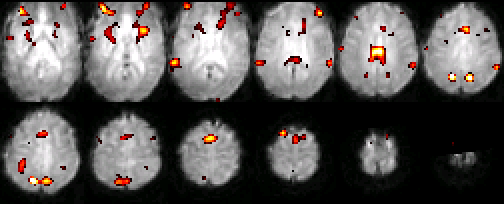
\includegraphics[width=4.0in]{./figures/Topic10/Fig10-17.png}
	\caption{A typical set of functional MRI images, where an activation map is overlaid on a normalized single subject functional scan.  The activation is related to the control of auditory spatial selective attention.}
	\label{Fig10-17}
\end{figure} 
 
\subsection{Small animal imaging and Molecular Imaging}

Tremendous strides have been made recently in understanding the molecular machinery that affects healthy and diseased mammalian tissues. These successes are due in large part to the use of small animals such as rats and mice, and numerous chemical methods for inducing conditions similar to diseases.   Also, small animals can be grown and bread rapidly to have special characteristics, such as chronic hypertension or obesity. Mice in particular can now be genetically manipulated so that they lack a specific gene from their genome. These “knock-out” animals allow scientists to test the role of specific genes in health and in disease.

Although most people would not object to killing these rodents in the interest of science, scientists are concerned with the constant need to sacrifice these animals in order to analyze those tissues containing the information of interest. This issue is particularly accentuated in experiments that aim at determining the time course of a disease, of the expression of a gene, or of the action of a new drug. The experiment begins with a cohort of animals with identical characteristics that are subjected simultaneously to the same intervention. Then, a number of them are sacrificed at every time point to quantitate of interest. The total number of animals used may depend on the number time points and on the used for every time, but typically require tens of animals. This number must be multiplied by two to account for control experiments, i.e. a comparative study where all conditions are duplicated without the intervention of interest.

The use of non-invasive imaging tools, such as CAT, PET, MRI, and optical scanners can in some instances provide an alternative to the continuous sacrifice of animals. For instance, the regression of a tumor triggered by a new drug could be quantified with one singlle animal if an imaging scanner (CAT or MRI) were used to image the tumor non-invasively at every-time point of the study. Gene expression could also be monitored live with a single animal if current assays for detecting this molecular process could be adapted so that they may be detected by PET or optical scanners. These compelling ideas have led to the development of imaging scanners that are optimized specifically for work with small rodents. Some of those imaging scanners are shown below.
\begin{figure}[!htb]
	\centering
	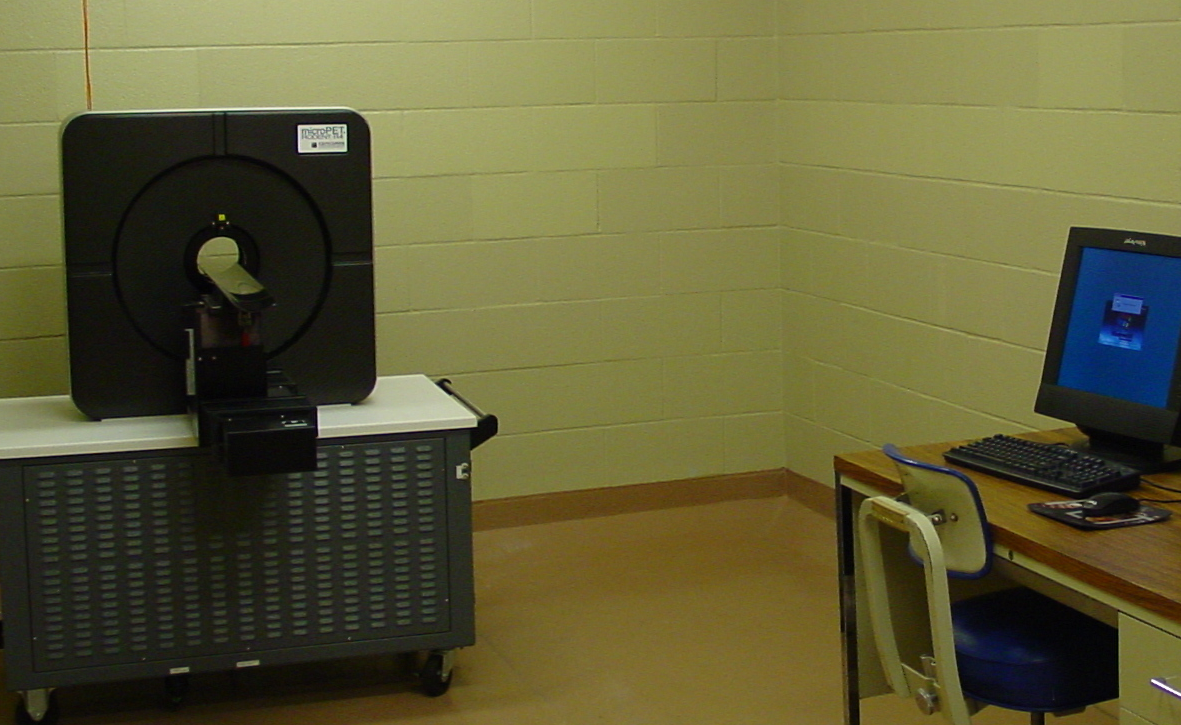
\includegraphics[height=2.1in]{./figures/Topic10/Fig10-18a.png}
	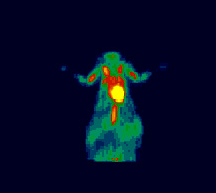
\includegraphics[height=2.1in]{./figures/Topic10/Fig10-18b.png}
	\caption{A microPET scanner and an image obtained with $^{18}$FDG. (Courtesy of (CG Kevil, TL Terry, and SC Barlow in LSU Health Sciences Center Shreveport.}
	\label{Fig10-18}
\end{figure} 	 
\begin{figure}[!htb]
	\centering
	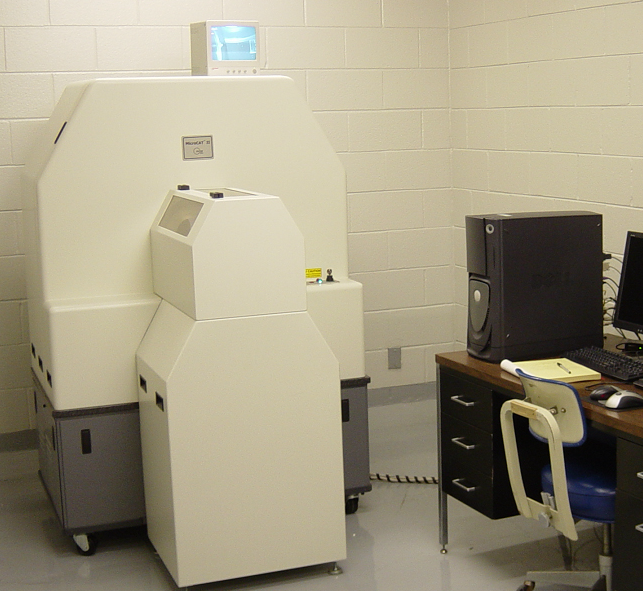
\includegraphics[height=2.1in]{./figures/Topic10/Fig10-19a.png}
	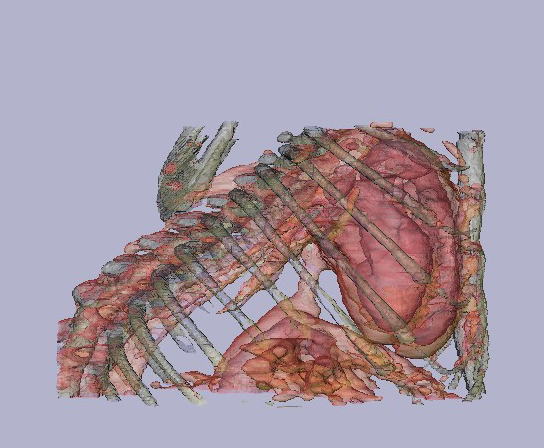
\includegraphics[height=2.1in]{./figures/Topic10/Fig10-19b.png}
	\caption{A microCT scanner and a 3D image obtained from a mouse thorax using a Fenestra contrast agent. (courtesy of JM Mathis, TL Terry, and SC Barlow -- from LSU health Sciences Center in Shreveport).}
	\label{Fig10-19}
\end{figure} 	 	 
\begin{figure}[!htb]
	\centering
	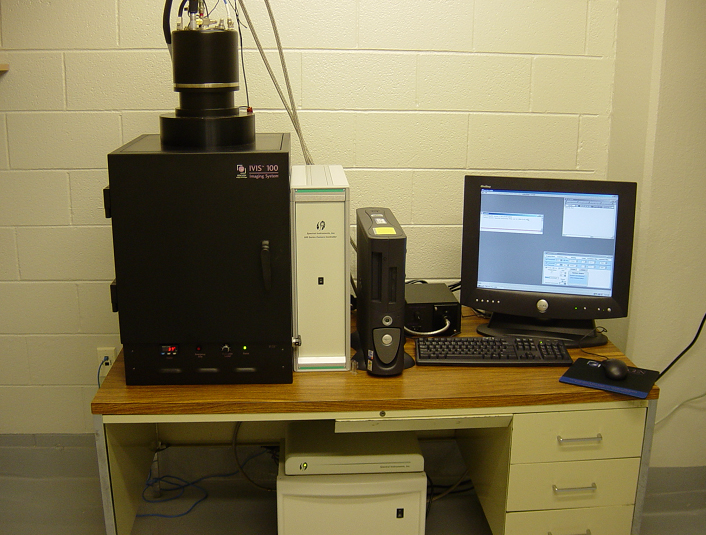
\includegraphics[height=2.1in]{./figures/Topic10/Fig10-20a.png}
	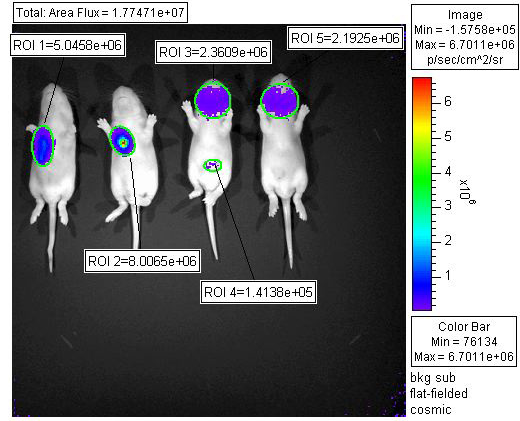
\includegraphics[height=2.1in]{./figures/Topic10/Fig10-20b.png}
	\caption{A bioluminescence CCD imaging camera and an image obtained with a luciferase virus. (Courtesy of  KD Ryman, WB Klimstra, TL Terry, and SC Barlow -- from LSU Health Sciences Center in Shreveport)}
	\label{Fig10-20}
\end{figure}




